\begin{equation}
    \begin{gathered}
        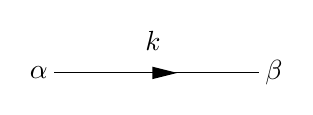
\begin{tikzpicture}[x=0.75pt,y=0.75pt,yscale=-1,xscale=1]
            %uncomment if require: \path (0,300); %set diagram left start at 0, and has height of 300
            
            %Straight Lines [id:da865326669998641] 
            \draw    (84,141.93) -- (136.7,141.93) ;
            \draw [shift={(138.7,141.93)}, rotate = 180] [fill={rgb, 255:red, 0; green, 0; blue, 0 }  ][line width=0.08]  [draw opacity=0] (12,-3) -- (0,0) -- (12,3) -- cycle    ;
            %Straight Lines [id:da20498887952582923] 
            \draw    (79.46,141.93) -- (177.93,141.93) ;
            
            % Text Node
            \draw (77.46,141.93) node [anchor=east] [inner sep=0.75pt]    {$\alpha $};
            % Text Node
            \draw (179.93,141.93) node [anchor=west] [inner sep=0.75pt]    {$\beta $};
            % Text Node
            \draw (122,120.4) node [anchor=north west][inner sep=0.75pt]    {$\boldsymbol{k}$};
            
            
            \end{tikzpicture}                
    \end{gathered} = - \frac{\delta_{\alpha \beta}}{\ii \omega_n - \xi_{\vb*{k}}},
\end{equation}